% Figure 4.3 (Session 4): the same block A on an open chain (one cut) and on a ring (two cuts).
% The image is rendered by figures/blender/s4_3_boundary_cuts.py; the coordinates of the labels come
% from figures/blender/out/boundary_cuts_anchors.tex. Compile with:
%   pdflatex boundary_cuts.tex ; result moves to ../mps_spin_chains/boundary_cuts.pdf
\documentclass[11pt,tikz,border=0pt]{standalone}
\usepackage{amsmath,amssymb,graphicx}
\usepackage{xcolor}
\definecolor{coursedark}{HTML}{1B2A4A}
\definecolor{costamber}{HTML}{B8620A}
\newlength{\figw}\setlength{\figw}{16.19cm}   % the text width of the notes (letter, 2.7 cm margins), so labels print at size

\begin{document}
\begin{tikzpicture}[lbl/.style={font=\small, text=coursedark}]
  \node[anchor=south west, inner sep=0pt] at (0,0)
    {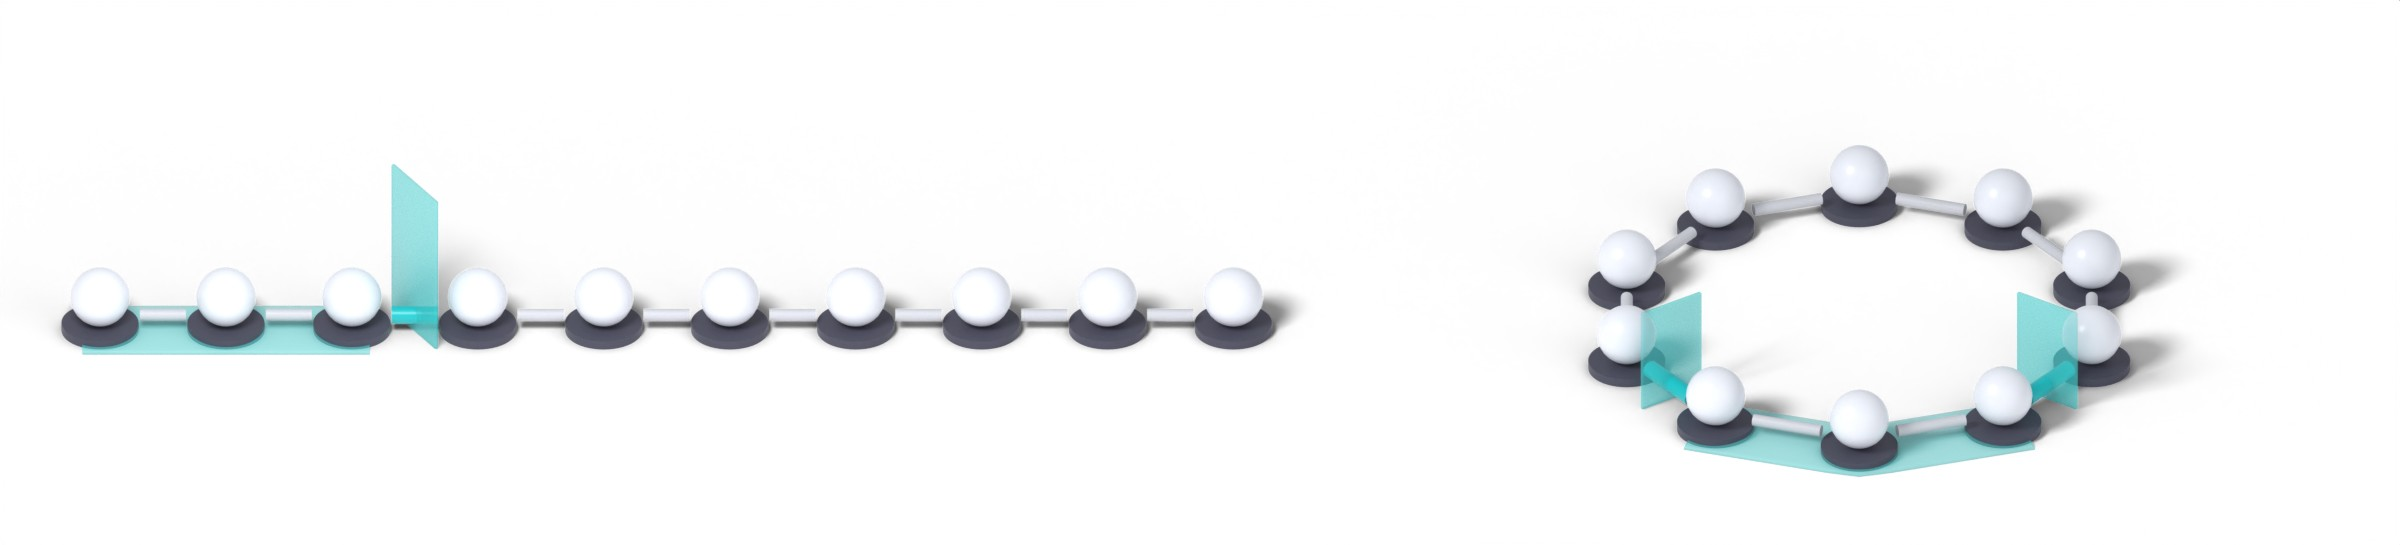
\includegraphics[width=\figw]{../blender/out/boundary_cuts.jpg}};
  %% written by figlib.py; x and y in units of the image width
\coordinate (a) at (0.0108\figw,0.1697\figw);
\coordinate (Aa) at (0.0941\figw,0.0741\figw);
\coordinate (cuta) at (0.1728\figw,0.1536\figw);
\coordinate (cutb0) at (0.8796\figw,0.0514\figw);
\coordinate (cutb1) at (0.6698\figw,0.0514\figw);
\coordinate (b) at (0.6111\figw,0.1697\figw);
\coordinate (Ab) at (0.7747\figw,0.0231\figw);

  \node[lbl, font=\normalsize, anchor=west] at (a) {(a)};
  \node[lbl, font=\normalsize, anchor=west] at (b) {(b)};
  \node[lbl, anchor=north] at (Aa) {$A$};
  \node[lbl, anchor=north] at (Ab) {$A$};
  \node[lbl, anchor=south] at (cuta) {cut};
  \node[lbl, anchor=north west] at (cutb0) {cut};
  \node[lbl, anchor=north east] at (cutb1) {cut};
\end{tikzpicture}
\end{document}
